\documentclass{beamer}
\usepackage[brazil]{babel}
\usepackage[utf8]{inputenc}
\usepackage[T1]{fontenc}
\usepackage{array}
\usepackage{listings}

\usetheme{Laughlin}

\begin{document}
\title{Seminário de Andamento de Doutorado - Extração de Dados Estruturados}
%\author[Roberto Panerai Velloso]{Orientando: Roberto Panerai Velloso \\
%Orientadora: Carina F. Dorneles \\ \{rvelloso, dorneles\}@gmail.com }
\author[Roberto Panerai Velloso]{Roberto Panerai Velloso, Carina F. Dorneles \\ 
\{rvelloso, dorneles\}@gmail.com}
%\date{\today}
\date{}
%\institute{Universidade Federal de Santa Catarina}
\institute{
%UFSC - Universidade Federal de Santa Catarina \\ PPGCC - Programa de
% Pós-Graduação em Ciência da Computação
\begin{figure}[H]
  \label{fig:logo1}
    
\includegraphics[scale=0.50]{img/brasao_ufsc_80.png}
    
\includegraphics[scale=0.30]{img/brasao_418.png}
\end{figure}
%\begin{figure}[H]
%  \label{fig:logo2}
%    
\includegraphics[scale=0.30]{brasao_ufsc_80.png}
%\end{figure}
}

\frame{
\titlepage
} 

\frame{\frametitle{Sumário}\tableofcontents}

\section{Introdução}
%\frame{\tableofcontents[currentsection]}

\subsection{Contexto}
\frame{\frametitle{Contexto}
\begin{itemize}
\item Obter informação estruturada (\textit{i.e.}, relacional) a partir de
fontes não estruturadas ou semiestruturadas.

\item Dados são disponibilizados na \textit{web} para serem consumidos por
pessoas, não por máquinas.

\item Motivação
\begin{itemize}
  \item realizar consultas com SQL;
  \item criar bases de dados para domínios específicos;
  \item enriquecer outras aplicações;
  \item criar taxonomias.
\end{itemize}
\end{itemize}
}

\subsection{Problema}
\frame{\frametitle{Extração de Dados Estruturados}
\begin{itemize} 
	\item Extração a partir de fontes semiestruturadas;
	\item Utilização de informação sintática;
	\item Requisitos de escalabilidade:
	\begin{itemize}
	  \item nível de supervisão;
	  \item generalidade;
	  \item precisão vs \textit{recall}. 
\end{itemize}
\end{itemize}
}

\subsection{Objetivo}
\frame{\frametitle{Objetivo Geral} 
O objetivo geral desta pesquisa é desenvolver um método automático (não
supervisionado) de extração de dados estruturados a partir de informação
semiestruturada contida em páginas \textit{web}.
}

\frame{\frametitle{Objetivos específicos}
\begin{itemize}
\item desenvolver um método de \textbf{segmentação} de um documento HTML que
identifique as regiões da página com conteúdo semiestruturado;
\item desenvolver um método de \textbf{filtragem} que identifique quais das
regiões semiestruturadas possuem conteúdo e quais possuem ruído (menus, \textit{template}, anúncios,
etc.);
\item desenvolver um método de estruturação da informação semiestruturada
identificada (\textit{e.g.} \textbf{alinhamento} de registros);
\item desenvolver um \textbf{\textit{framework}} de extração estruturada;
\item criar \textbf{\textit{datasets}} com ampla cobertura para avaliação de
métodos de extração;
\end{itemize}
}

\subsection{Contribuições}
\frame{\frametitle{Contribuições}
\begin{itemize}
  \item desenvolvimento de um novo método de extração estruturada;
  \item criação de \textit{datasets} com ampla cobertura para avaliação de
  métodos de extração estruturada;
  \item proposição de novas métricas;
  \item publicação dos resultados da pesquisa em eventos e periódicos;
  \item desenvolvimento de um \textit{framework} de extração estruturada. 
\end{itemize}
}

\section{Trabalhos Relacionados} 
\frame{\frametitle{Trabalhos Relacionados}
\begin{itemize}
\item Poucas implementações disponíveis;
\item Alguns datasets disponíveis; 
\item Três principais abordagens identificadas:
\begin{itemize}
  \item extração de tabelas e listas;
  \item extração a partir de uma única página;
  \item extração a partir de múltiplas páginas.
\end{itemize}
\end{itemize}
}

\subsection{Tabelas e Listas}
\frame{\frametitle{Extração de Tabelas e Listas}
Abordagens fazem suposições \textbf{fortes} a respeito da entrada.
\begin{itemize}
  \item webtables google (\texttt{<table>}) (2008);
  \item webtables M\$ (\texttt{<table>}) (2012);
  \item ListExtract (\texttt{<ol/ul/etc.>}) (2009);
  \item Tegra (ListExtract da M\$) (\texttt{<ol/ul/etc.>}) (2015);
  \item \textit{Top-k pages} (\textit{template} fixo) (2013).
\end{itemize}
}

\subsection{Única Página}
\frame{\frametitle{Extração a partir de uma única página}
Buscam padrões no HTML/DOM para encontrar os registros. Ao menos dois registros
devem existir para ser possível a extração.
Algumas abordagens ``gerais'':
\begin{itemize}
  \item Abordagens não visuais: MDR, NET, TPC (2003 - 2009);
  \item Abordagens visuais: DEPTA, ViPER, ClustVX, AutoRM, (CHU et al., 2015b)
  (2005 - 2015);
\end{itemize}
}

\subsection{Múltiplas Páginas}
\frame{\frametitle{Extração a partir de múltiplas páginas}
Utilizam uma ``amostra'' do \textit{template} do \textit{site} para treinamento.
São capazes de extrair conteúdo de páginas com apenas um registro.
(\textit{i.e., páginas de detalhe}).
\begin{itemize}
  \item RoadRunner (2001);
  \item ExAlg (2003);
  \item FiVaTech (2010).
\end{itemize} 
}

\section{Proposta}

\subsection{Características}
\frame{\frametitle{Características}
\begin{itemize}
  \item Independente de domínio;
  \item Independente de características da linguagem HTML; 
  \item Não dependa de bases de dados e/ou definições \textit{a priori}.
  \item Totalmente automática;
  \item Necessite de apenas uma página (ao invés de um conjunto de páginas);
  \item Não dependa de treinamento;
  \item Computacionalmente eficiente.
\end{itemize}
}

\subsection{Suposições}
\frame{\frametitle{Suposições}
\begin{enumerate}
\item \textbf{Segmentação}: diferentes
regiões de uma página HTML são formatadas de maneiras diferentes, justamente
para que haja distinção entre elas, portanto serão formadas por conjuntos de \textit{tag
paths} diferentes, caso contrário não haveria diferença visual
significativa entre as regiões de uma página;
\item \textbf{Registros}: regiões com conteúdo semiestruturado são compostas por
conjuntos de registros contíguos e com estrutura semelhantes, 
descritos por sequências de \textit{tag paths} semelhantes sendo, portanto, regiões cíclicas.
\end{enumerate} 
}

\subsection{Tag Paths}
\frame{\frametitle{$Tag$ $paths$}
\begin{figure}[H]
  \caption{Construção da sequência de $tag$ $paths$ (TPS) a partir do HTML.}
  \label{fig:ex1}
  \centering
    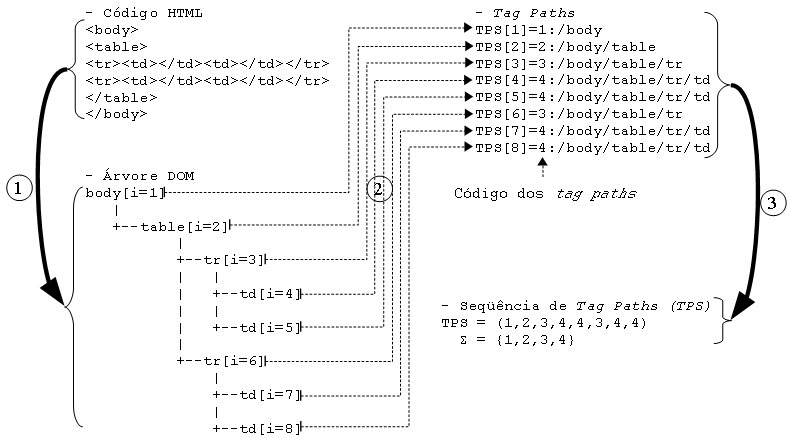
\includegraphics[scale=0.45]{img/example1-pt.jpg}
\end{figure}
}

\section{Cronograma}
\end{document}
